\section{Noise Effect}
In a real enviroment system nodes are affected by measurement error. One error source is represented by the noise contribution on the signal measurement.
For this project a white noise with normal distribution have been been considered with a maximum power of 100mW (taken from the EIRP maximum wi-fi irradiance 
in the Europian Union) and assuming a 20mA consumption by the sensor. 

\begin{figure}[H]
        \centering
        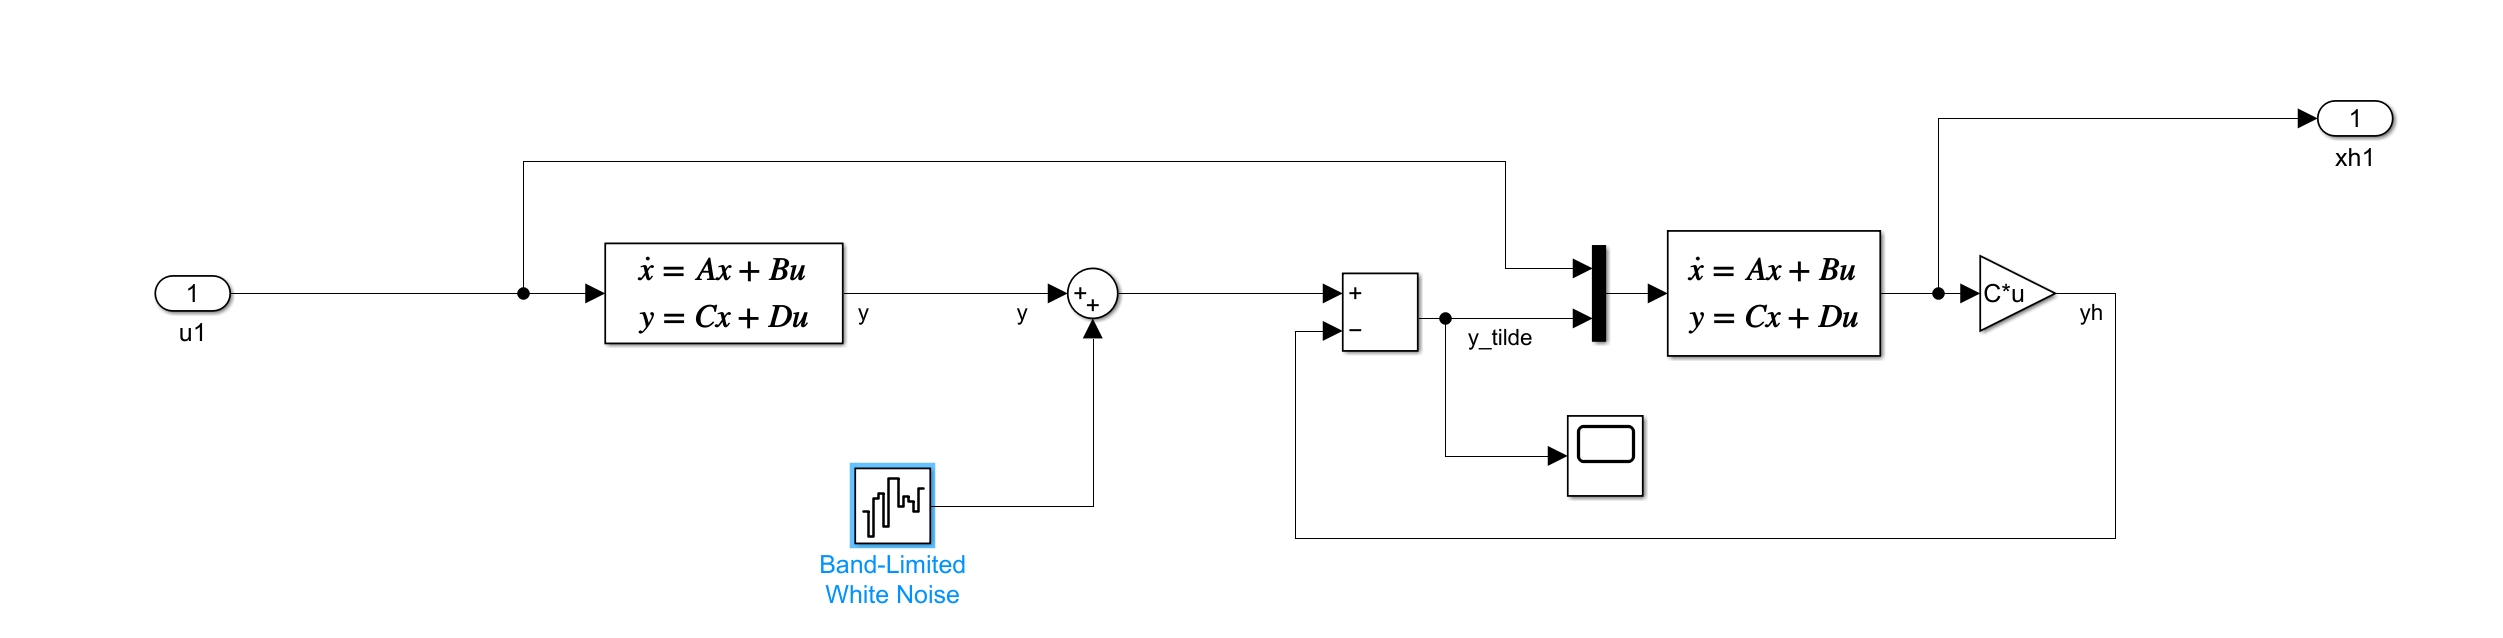
\includegraphics[width=\textwidth]{img/node_structure_w_noise.PNG}
        \caption{IST}
    \caption{Node structure with noise implementation}
\end{figure}

We analyzed the effect of the noise in the case of distribuited observer and when we rely only on the local observer without neighborhood contribution.
What we observed is that the noise attenuation is similar in either cases with the first case better at attenuating the velocity and the second one, which relies on the 
local observed, better at attenuating the vertical position.

\begin{figure}[H]
    \begin{subfigure}{0.45\textwidth}
        \centering
        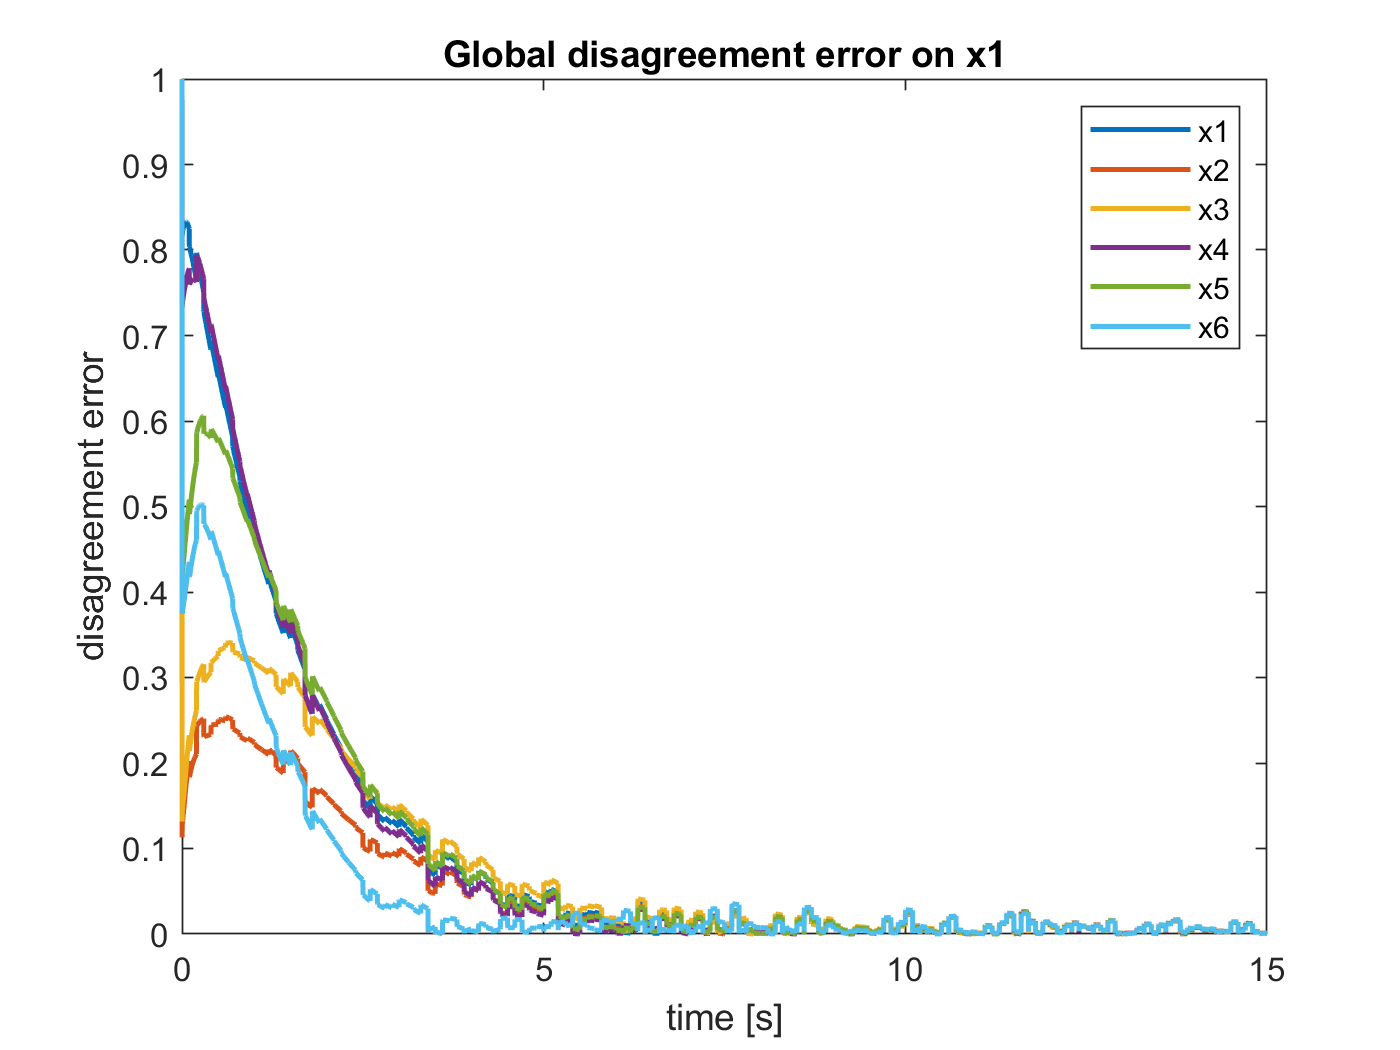
\includegraphics[width=\textwidth]{img/dist/global_error_x1_noise_dist.png}
        \caption{Distributed observer}
    \end{subfigure}
    \hfill
    \begin{subfigure}{0.45\textwidth}
        \centering
        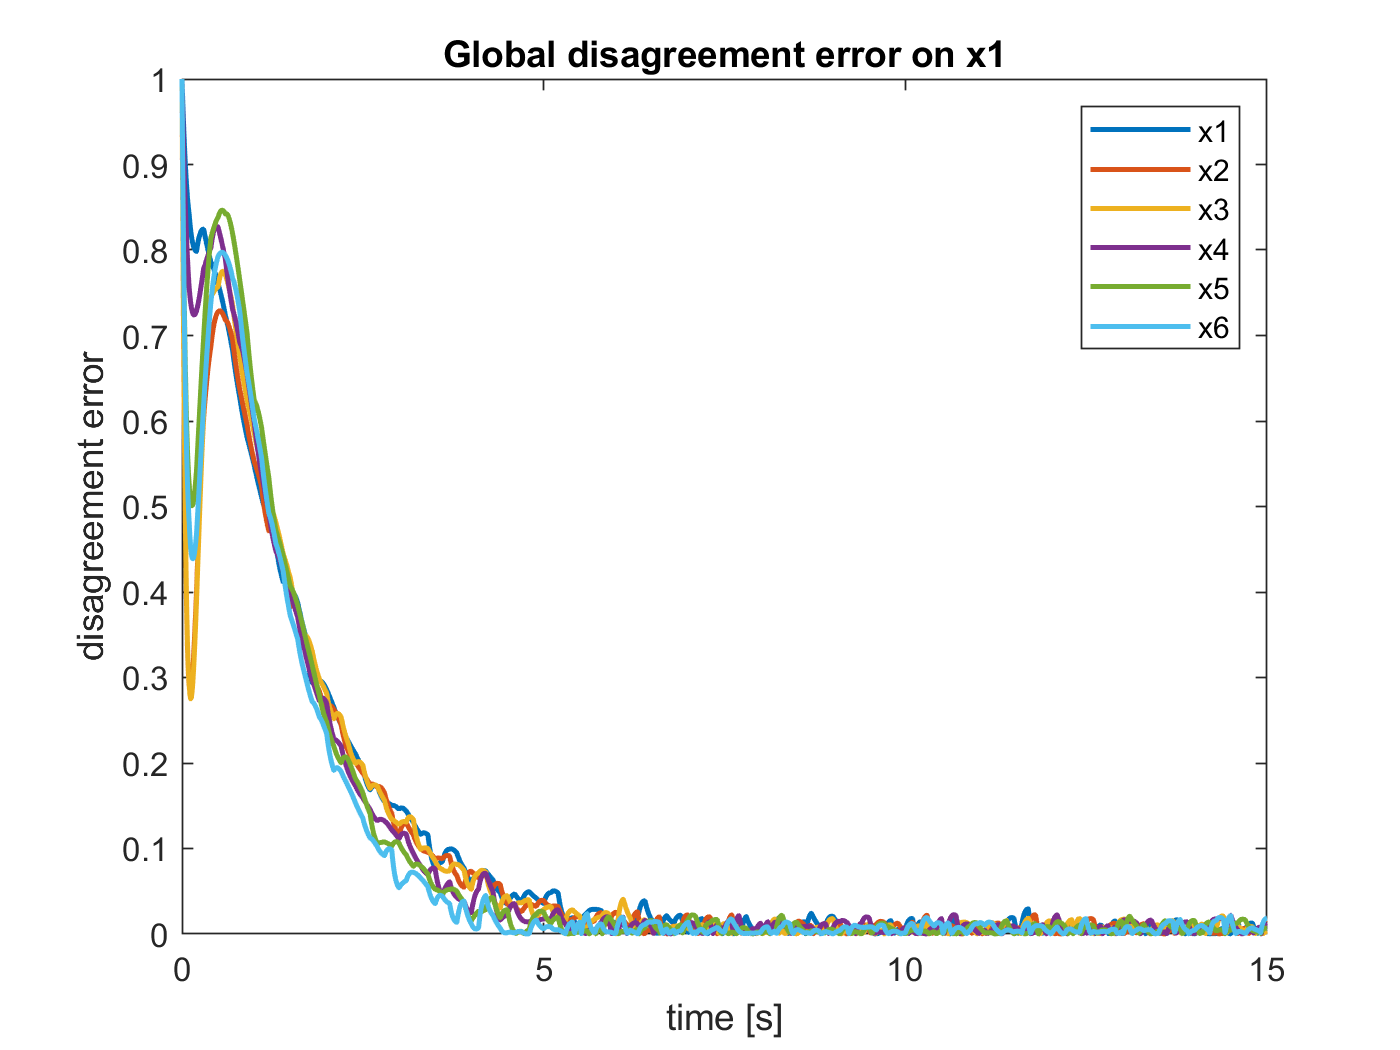
\includegraphics[width=\textwidth]{img/local/global_error_x1_noise_local.png}
        \caption{Local Observer}
    \end{subfigure}
    \caption{Comparison on vertical position (x1) cumulative disagreement error}
    \label{fig:x1_error}
\end{figure}

\begin{figure}[H]
    \begin{subfigure}{0.45\textwidth}
        \centering
        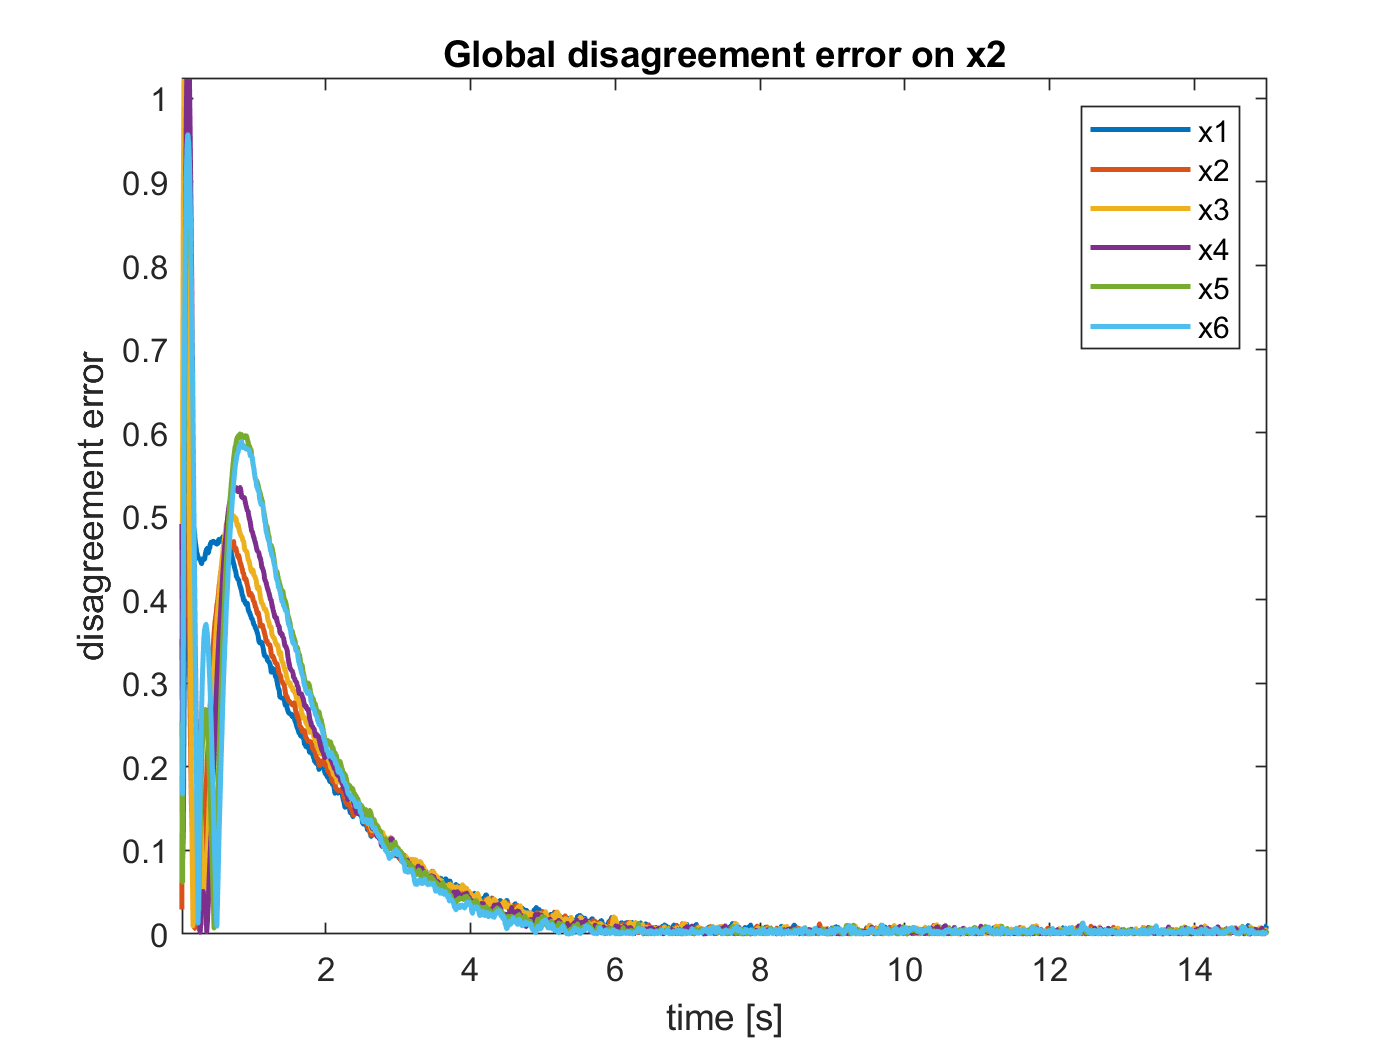
\includegraphics[width=\textwidth]{img/dist/global_error_x2_noise_dist.png}
        \caption{Distributed observer}
    \end{subfigure}
    \hfill
    \begin{subfigure}{0.45\textwidth}
        \centering
        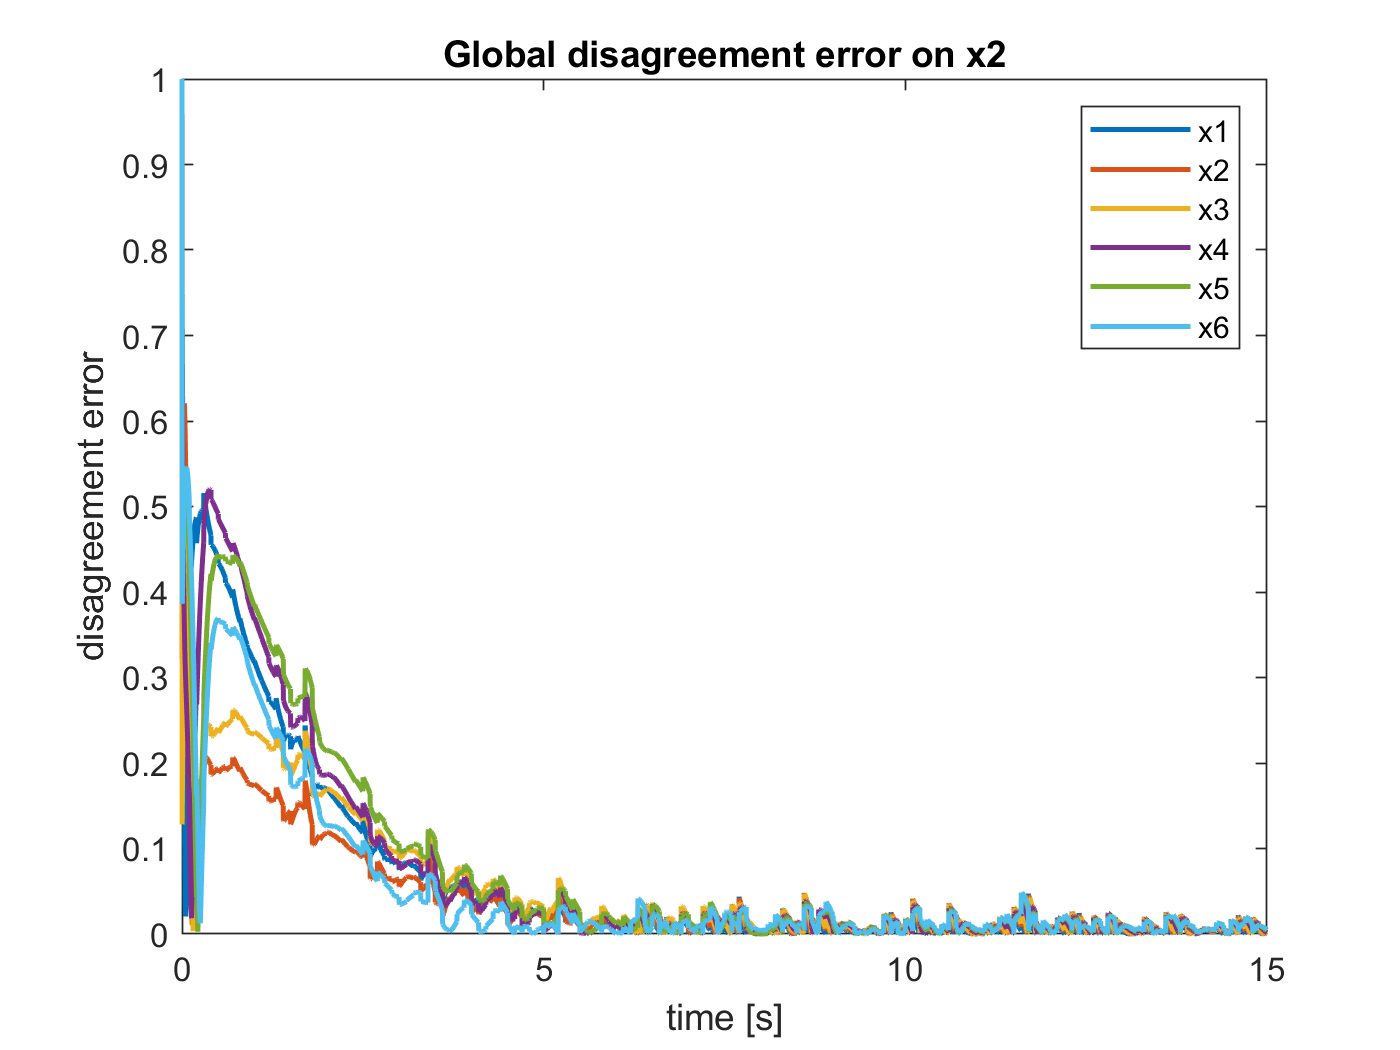
\includegraphics[width=\textwidth]{img/local/global_error_x2_noise_local.png}
        \caption{Local Observer}
    \end{subfigure}
    \caption{Comparison on velocity (x2) cumulative disagreement error}
    \label{fig:x2_error}
\end{figure}

As can be seen in \ref{fig:SBVF} the results have been performed using as reference a sinusoidal signal.
We observed the same behavior also with a constant reference.
In conclusion we can say that the network can succesfully manage some noise during the measurement process 
but it isn't able to completely cancel it.

\begin{figure}[H]
    \begin{subfigure}{0.45\textwidth}
        \centering
        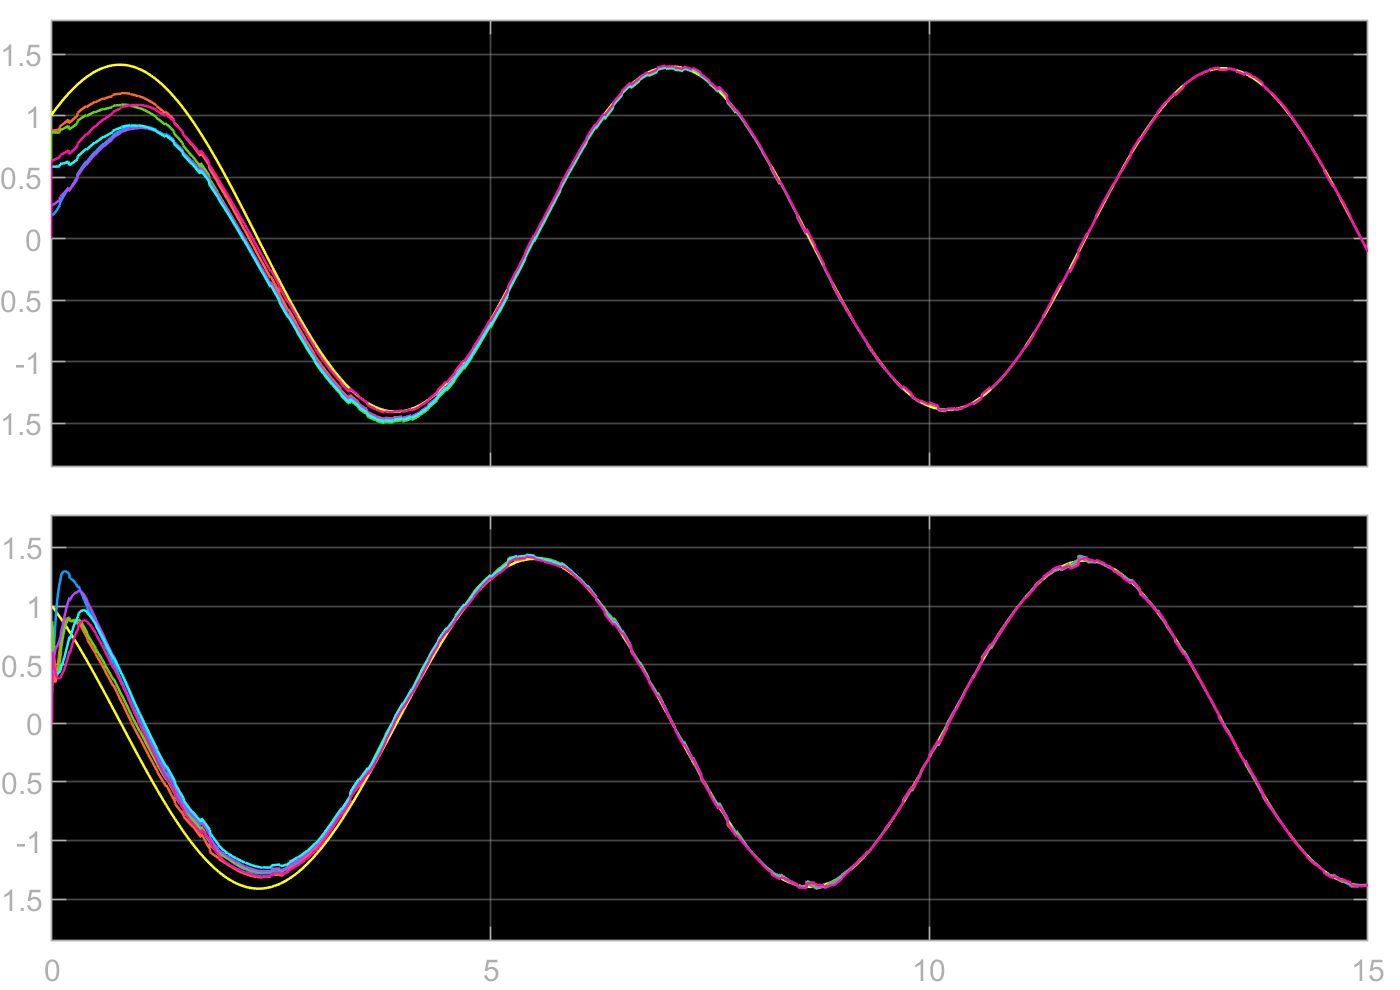
\includegraphics[width=\textwidth]{img/dist/dist_SBVF.png}
        \caption{Distributed observer}
    \end{subfigure}
    \hfill
    \begin{subfigure}{0.45\textwidth}
        \centering
        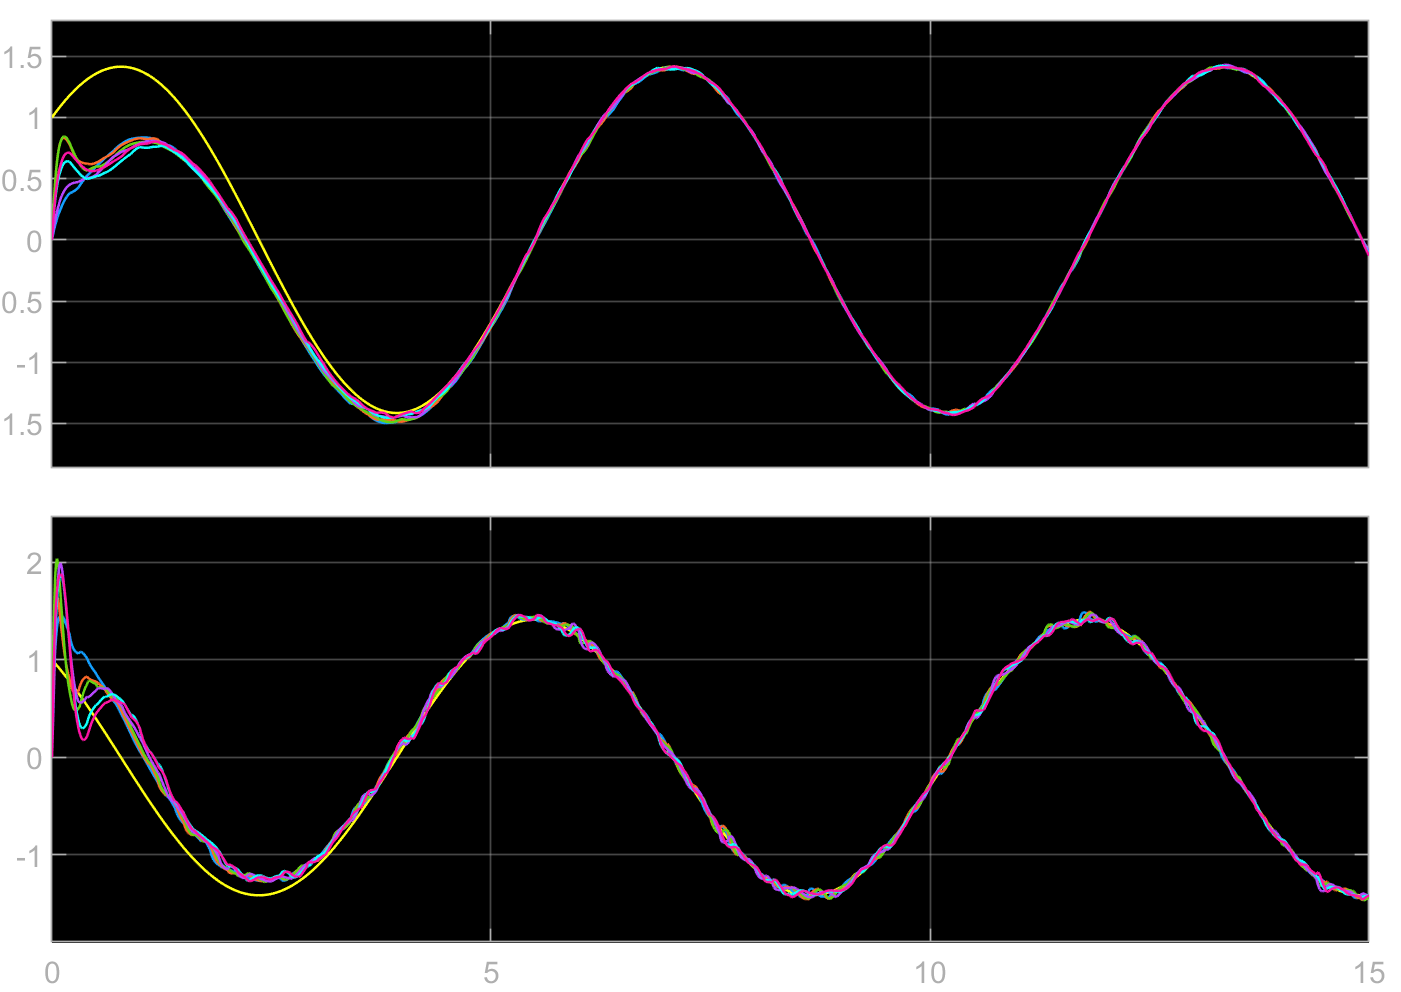
\includegraphics[width=\textwidth]{img/local/local_SBVF.png}
        \caption{Local Observer}
    \end{subfigure}
    \caption{Sinusoidal reference signal from $S_0$}
    \label{fig:SBVF}
\end{figure}